%
% This is file `dlrbeamer.tex',
% it includes examples for a DLR beamer template.
%
%
% REVISIONS:    2022-08-31 initial release (klem_ja)
%
% Contact       Jannik Klemm,  Jannik.Klemm@dlr.de
% Copyright (C) 2008-2022 DLR                                   __/|__	%                                                              /_/_/_/	  
%                                                                |/ DLR      
\RequirePackage{currfile}
% New design should show the text on the top
\documentclass[aspectratio=169,t]{beamer}

% Some default packages
\usepackage[english]{babel}
\usepackage[utf8]{inputenc}
\usepackage[T1]{fontenc}
\usepackage{qrcode}
\usepackage{tikz}
\usetikzlibrary {shapes.geometric}
\usepackage{pgfplots}
\usepackage{pgfplotstable}
%\pgfplotsset{compat=1.9,
	%title style={color=dlrdarkblue},
	%tick label style = {color=dlrdarkblue},
	%every axis label = {color=dlrdarkblue},
	%legend style,
	%label style = {color=dlrdarkblue}
%}
%\tikzset{cross/.style={cross out, draw=black, minimum size=2*(#1-\pgflinewidth), inner sep=0pt, outer sep=0pt},
	%default radius will be 1pt. 
	%cross/.default={1pt}}

% DLR Layout
%\usetheme[beamertools={fixblocktitle=false}, professionalfonts]{dlr}
%Select Blue, Green or Yellow as color
\usetheme[helvetica,nobeamertools,nonavigation,color=Blue]{Boadilla}

% Load a color scheme for blocks
\usecolortheme{orchid}

% Titel and author
\title{Wasserstoff für Deutschland}
\subtitle{} 
\date{29.02.2024}
\author{}


% Add additional logo
%\addlogoFL{{\includegraphics[height=24pt]{UzK_black.png}}}
%\addlogoTP{{\includegraphics[height=40pt]{UzK_black.png}}}

%%%%My colors
% SFC refienemnt colors
\definecolor{blue1}{RGB}{25,45,68}
\definecolor{blue2}{RGB}{29,51,78}
\definecolor{blue3}{RGB}{32,58,87}
\definecolor{blue4}{RGB}{36,64,97}
\definecolor{blue5}{RGB}{49,79,113}
\definecolor{blue6}{RGB}{64,94,129}
\definecolor{blue7}{RGB}{81,110,144}
\definecolor{blue8}{RGB}{100,128,160}
\definecolor{blue9}{RGB}{121,146,176}
\definecolor{blue10}{RGB}{143,166,192}
\definecolor{blue11}{RGB}{168,187,208}
\definecolor{blue12}{RGB}{195,208,223}
\definecolor{blue13}{RGB}{224,231,239}


\begin{document}
	
	% Maketitle
	\maketitle
	
	
	%---------------------------------
	

	
	%---------------------------------
	\begin{frame}
		\frametitle{Grober Überblick übers Projekt}
		\vspace*{0mm}
		\begin{itemize}
			\item Wollen das beschränkte Stromnetz Deutschlands modellieren
			\begin{itemize}
				\item [$\rightarrow$] Um Wasserstoffnetzwerk ergänzen
			\end{itemize}
		\item Gefälle von Nord- zu Süddeutschland bzgl. Stromproduktion und -verbrauch
		\begin{itemize}
			\item [$\rightarrow$] Verteilung von importiertem Strom
		\end{itemize}
		\item Für welche Gegebenheiten lohnt sich dieses Wasserstoffnetz?
		\item Aktuell: Stromtrassen als Lösung
		\item Problem: ungenutzter Strom 
		\item Lösung: Strom in Form von Wasserstoff speichern und transportieren 
		
			 
		\end{itemize}
		
			
		
	\end{frame}
			
	%---------------------------------
	
	
	\begin{frame}
		\frametitle{Erste Schritte}
		\vspace*{0mm}
		\begin{minipage}{1\linewidth}
			\begin{minipage}{.5\linewidth}
				\begin{itemize}
					\item Modellierung des Stromnetzes in Deutschland
					\item Bundesländer als Knoten eines gerichteten Graphens in Python
					\item einfaches Beispiel mit vereinfachten Annahmen
					\item ausschließlich Sonnen- und Windenergie
				\end{itemize}
			\end{minipage}
			\hfill
			\begin{minipage}{.5\linewidth}
				\centering
				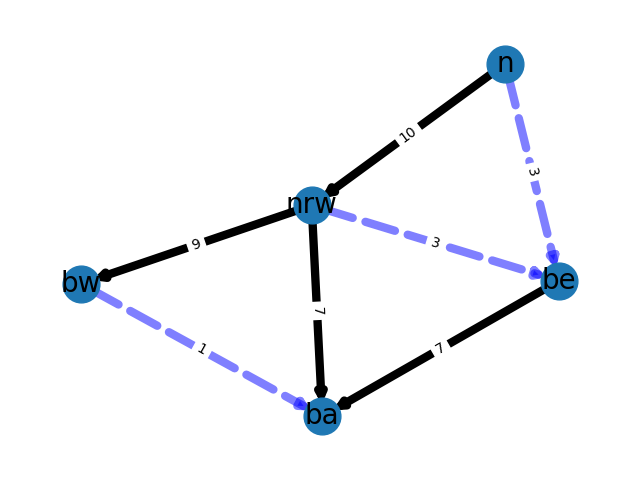
\includegraphics[width=.7\linewidth]{Example_graph.png}
				
			\end{minipage}
		\end{minipage}	
		
	\end{frame}

	%---------------------------------
\begin{frame}
	\frametitle{Annahmen}
	\vspace*{0mm}
	\begin{minipage}{1\linewidth}
		\begin{minipage}{.3\linewidth}
			\begin{itemize}
				\item Verbrauch
				\item 1 toe = 11.63 megawatt-hours (MWh)
			\end{itemize}
		\end{minipage}
		\hfill
		\begin{minipage}{.7\linewidth}
			\centering
			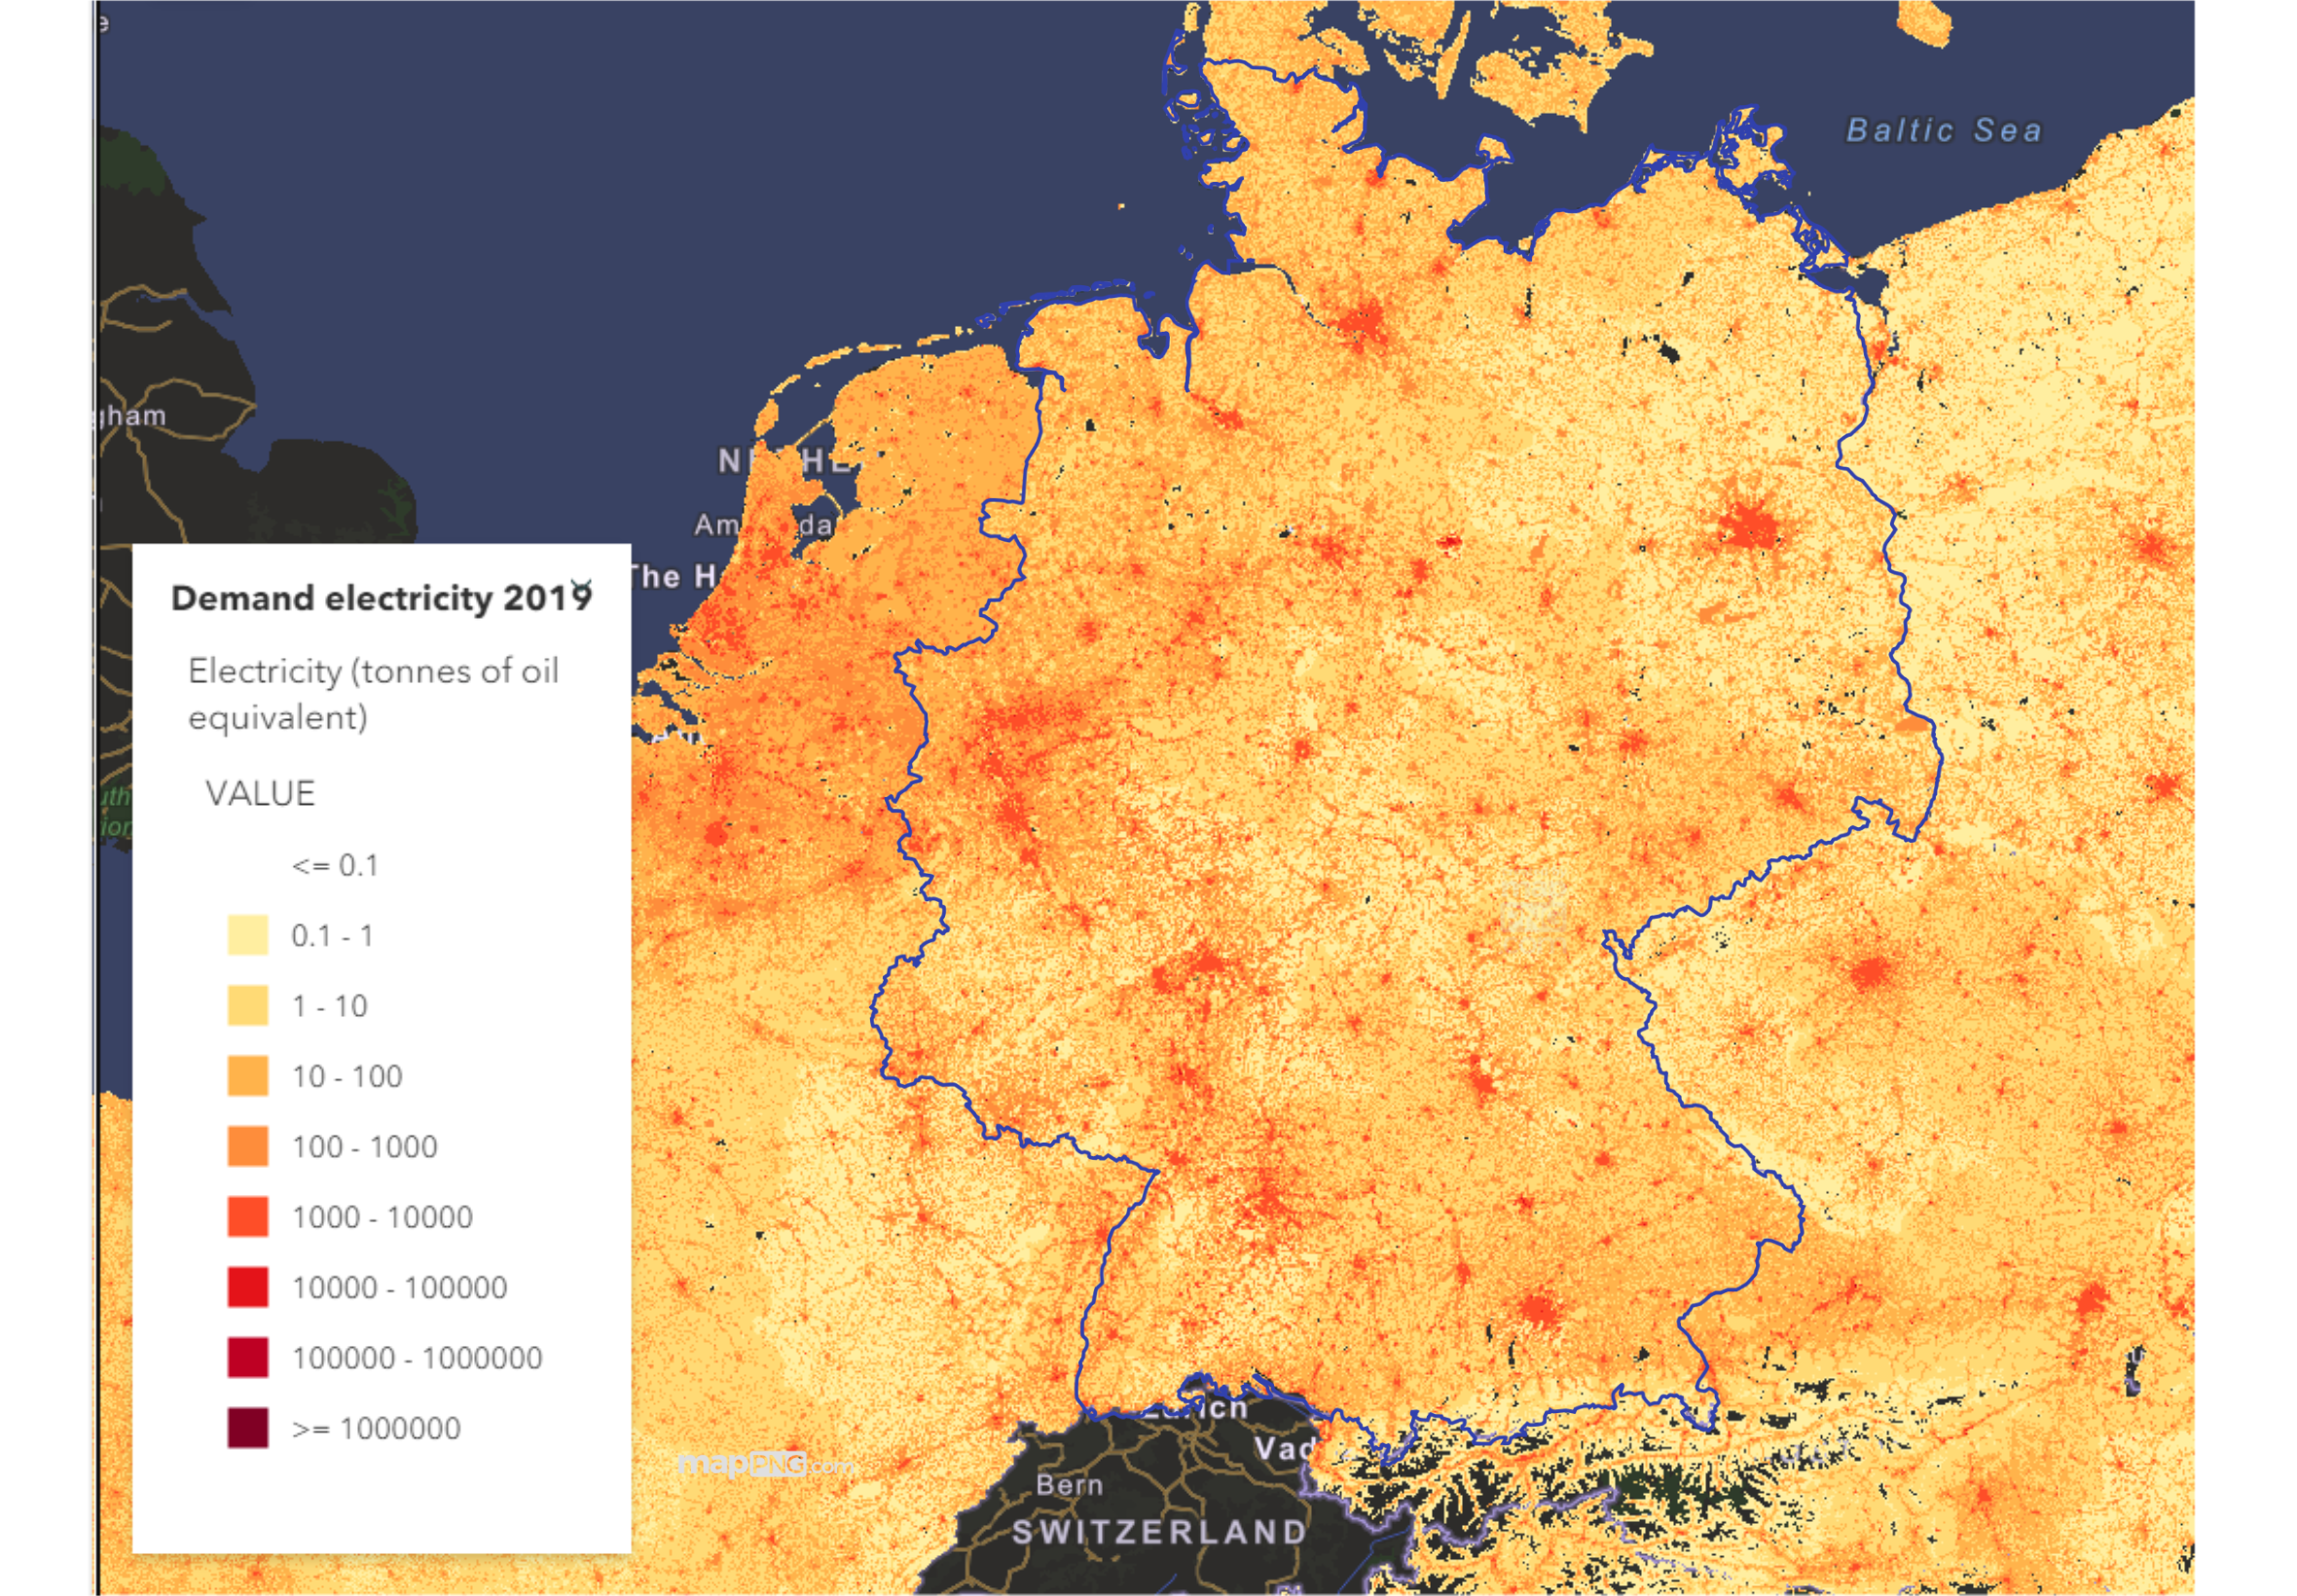
\includegraphics[width=.9\linewidth]{Deutschland_Bedarf.png}
			
		\end{minipage}
	\end{minipage}	

\vspace*{4mm}
	Quelle: https://energy-industry-geolab.jrc.ec.europa.eu/energy-atlas/
	
\end{frame}

	%---------------------------------


\begin{frame}
	\frametitle{}
	
	\vspace*{-2mm}
	%Verbrauch: https://www.statistikportal.de/de/ugrdl/ergebnisse/energie/pev#5238
	%Erzeugung: https://www.statistikportal.de/de/ugrdl/ergebnisse/energie/swe#5897
	\vspace*{0mm}
\end{frame}
%---------------------------------
	

	%---------------------------------
	\begin{frame}
		\frametitle{Weitere Vorgehensweise}
		\vspace*{0mm}
			\begin{minipage}{1\linewidth}
			\begin{minipage}{.5\linewidth}
				\begin{itemize}
					\item größeres Modell
					\begin{itemize}
						\item Deutschland aufgeteilt in 16 Bundesländer
					\end{itemize}
					\item 
					\item
					\item Powerflow Equations
				\end{itemize}
			\end{minipage}
			\hfill
			\begin{minipage}{.5\linewidth}
				\centering
				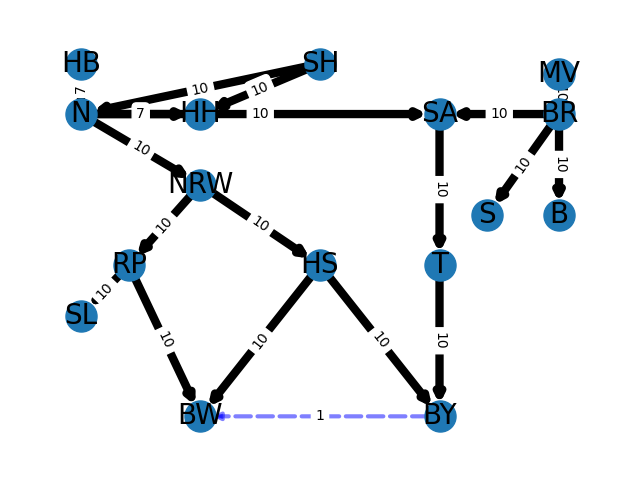
\includegraphics[width=.8\linewidth]{Example_graph_2.png}
				
			\end{minipage}
		\end{minipage}	
	
			
	\end{frame}
	%---------------------------------
	
	
	\begin{frame}
		\frametitle{Powerflow Equations}
		
		\vspace*{-2mm}
		
		
		\vspace*{0mm}
	\end{frame}
	%---------------------------------
	
	

	
	
	\begin{frame}
		\frametitle{Ausblick}
		
		\vspace*{6mm}
		\begin{itemize}
			\item weiter Daten suchen 
			\item Stahlindustrie betrachten
		\end{itemize}
			
		
	\end{frame}
	
	
	
	%---------------------------------
	
	
	
	
\end{document}
% eof
